\documentclass[12pt,a4paper,oneside]{book}
\usepackage[utf8]{inputenc}
\usepackage[english]{babel}
\usepackage[T1]{fontenc}
\usepackage[hidelinks]{hyperref}
\usepackage{amsmath}
\usepackage{amsfonts}
\usepackage{amssymb}
\usepackage{algorithm}
\usepackage[noend]{algpseudocode}
\usepackage{listings}
\usepackage{pdfpages}
\usepackage{indentfirst}
\usepackage{titlesec}
\usepackage{tocloft}
\usepackage{setspace}
\usepackage{siunitx}
\usepackage{graphicx}
\usepackage{tabularx}
\usepackage{array}
\usepackage{multirow}
\usepackage{multicol}
\usepackage{threeparttable}
\usepackage{fixltx2e}
\graphicspath{ {./figures/} }
%\usepackage{natbib}
\usepackage[left=3.5cm,right=2cm,top=2.5cm,bottom=2.5cm]{geometry}
\setstretch{1.5} %riadkovanie 1.5
\titleformat{\chapter}{\normalfont\huge\bfseries}{\thechapter}{20pt}{\normalfont\huge\bfseries}
\setcounter{tocdepth}{3}
\setcounter{secnumdepth}{3}
\newtheorem{definition}{Definition}

\newcommand\mytitle{Software for isometric gene tree reconciliation}
\newcommand\mythesistype{Master's thesis}
\newcommand\myauthor{Bc. Dominika Mihálová}
\newcommand\myadvisor{doc. Mgr. Bronislava Brejová, PhD.}
\newcommand\myplacedate{Bratislava, 2021}
\newcommand\myuniversity{COMENIUS UNIVERSITY IN BRATISLAVA}
\newcommand\myfaculty{FACULTY OF MATHEMATICS, PHYSICS AND INFORMATICS}
\newcommand{\sub}[1]{$_{\text{#1}}$}
\newcommand{\reference}[1]{č.~\ref{#1}}
\newcommand{\imageHeight}{150px}
\renewcommand{\cftchapleader}{\cftdotfill{\cftdotsep}}

\begin{document}
\sloppy
%obal
\frontmatter
\thispagestyle{empty}
\noindent
\begin{minipage}{\textwidth}
	\begin{center}
		\textbf{\myuniversity \\
		\myfaculty}
	\end{center}
\end{minipage}

\vfill
\begin{center}
	\begin{minipage}{0.8\textwidth}
		\centering{\textbf{\Large\MakeUppercase{\mytitle}}} \\
		\centering{\mythesistype}
	\end{minipage}
\end{center}
\vfill
2020 \hfill
\myauthor
\eject 

%titulná strana
\thispagestyle{empty}
\noindent
\begin{minipage}{\textwidth}
	\begin{center}
		\textbf{\myuniversity \\
		\myfaculty}
	\end{center}
\end{minipage}
\vfill

\begin{center}
	\begin{minipage}{0.8\textwidth}
		\centering{\textbf{\Large\MakeUppercase{\mytitle}}} \\
		\centering{\mythesistype}
	\end{minipage}
\end{center}
\vfill
\begin{tabular}{l l}
	Study programme: & Applied Computer Science\\
	Field of study: & Computer Science\\
	Department: & Department of Computer Science\\
	Supervisor: & \myadvisor
\end{tabular}
\vfill
\noindent
\myplacedate \hfill
\myauthor
\eject 

%zadanie - pojde obrazok
%\chapter*{Thesis assignment}
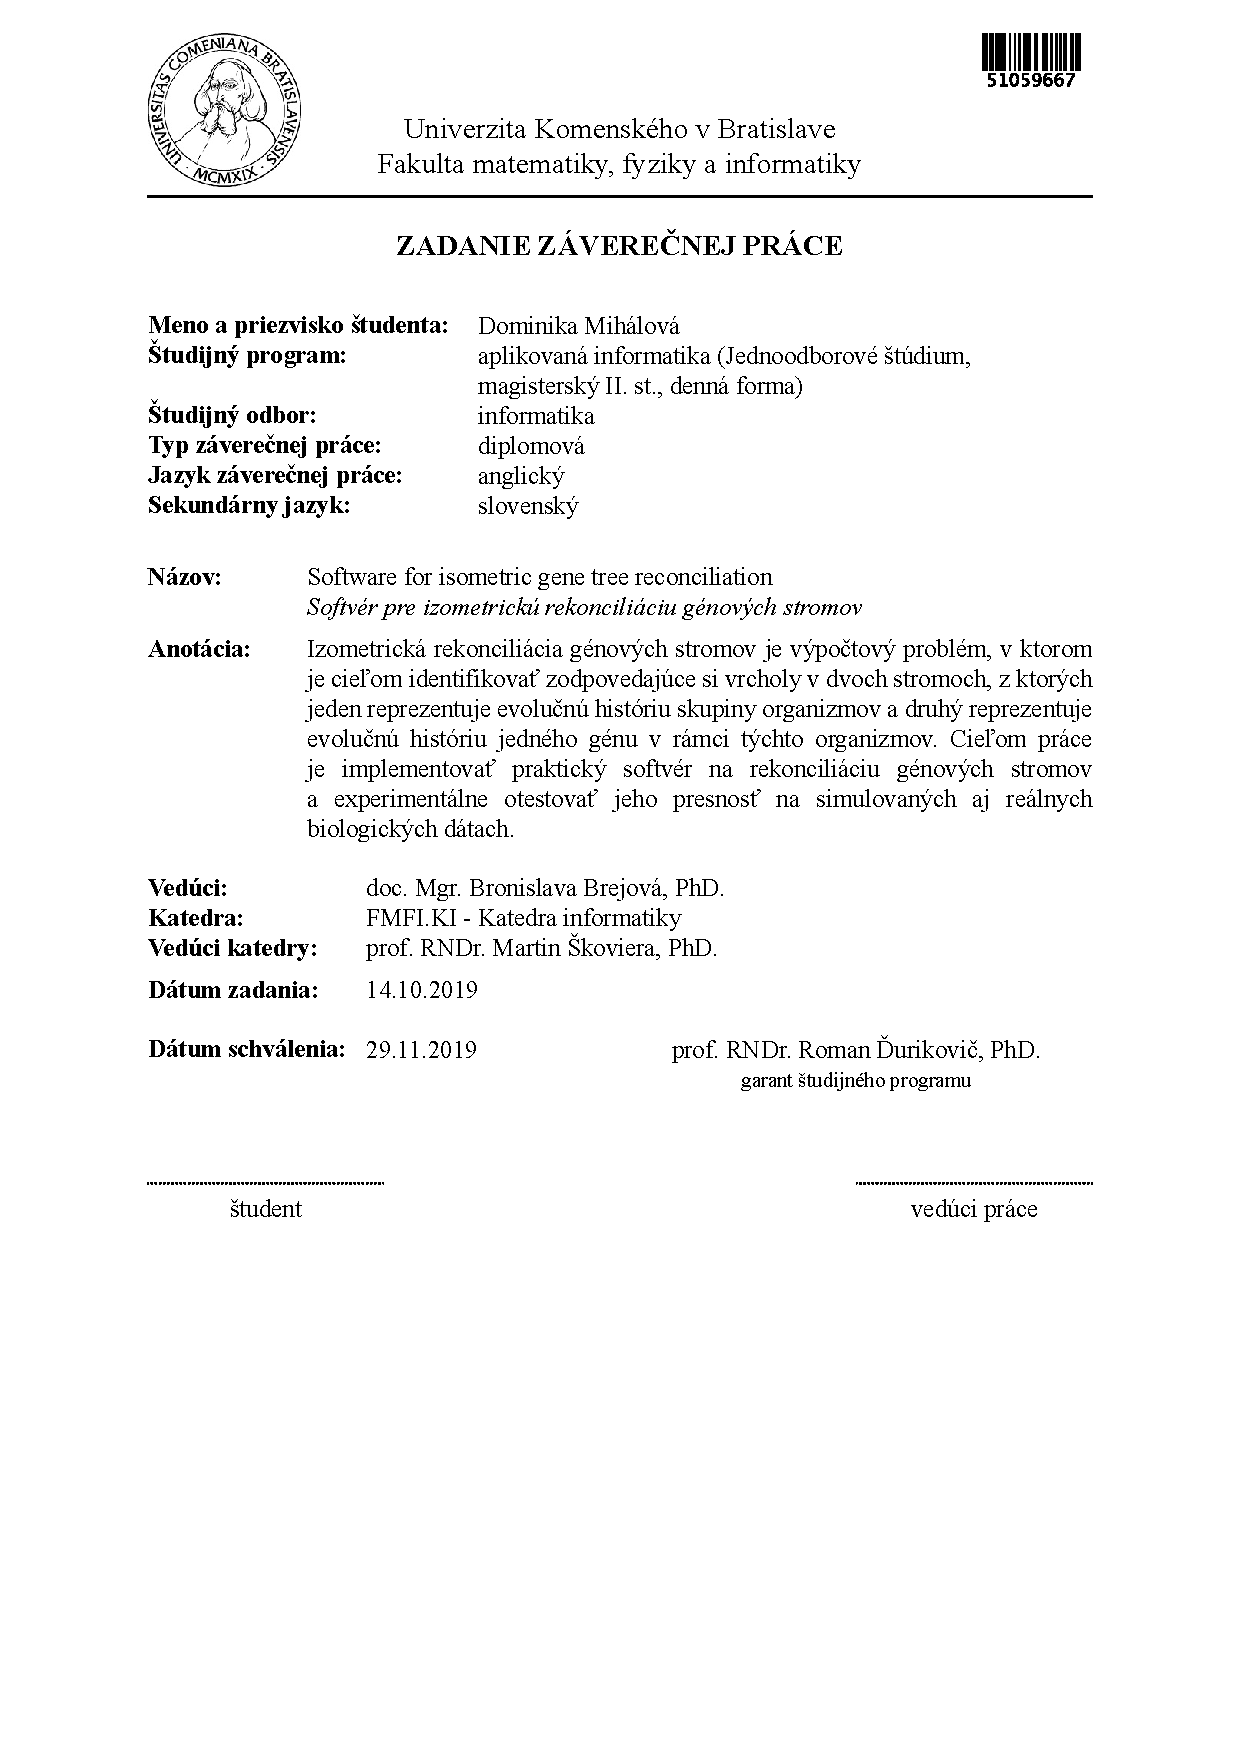
\includepdf{zadanie-zp.pdf}
\vfill\eject 

%sk abstrakt
\chapter*{Abstrakt}

Evolučná história môže byť zobrazená fylogenetickými stromami. Používame dva typy fylogenetických stromov: strom druhov a génový strom. Strom druhov predstavuje vývoj druhu a genový strom predstavuje vývoj jedného génu. Izometrická rekonciliácia génových stromov je problém mapovania génového stromu na~strom druhov so~zachovaním dĺžok hrán. V tejto práci sa zameriavame na~riešenie problému izometrickej rekonciliácie génových stromov s~nepresnými dĺžkami hrán. Nadviazali sme na~predchádzajúci výskum a predstavujeme dva algoritmy, ktoré sú implementované v~softvéri v kombinácii s~algoritmami z~predchádzajúceho výskumu. Implementovaný softvér je experimentálne testovaný na simulovaných a reálnych biologických dátach a porovnávaný s~inými softvérmi.
\\\\
\textbf{Kľúčové slová:} izometrická rekonciliácia génových stromov, nepresné dĺžky hrán, fylogenetický strom
\vfill\eject 

%en abstrakt
\chapter*{Abstract}

Evolutionary history can be presented by phylogenetic trees. We use two types of~phylogenetic trees: species tree and gene tree. A~species tree represents the evolution of a~species and a~gene tree represents the evolution of one gene. Isometric gene tree reconciliation is a~problem of mapping the gene tree to species tree with preserving the edge lengths. In this work, we focus on solving the problem of isometric gene tree reconciliation with inexact branch lengths. We built on the previous research and present two algorithms that are implemented in software in combination with~algorithms from previous research. The implemented software is experimentally tested on simulated and real biological data and compared with other software.
\\\\
\textbf{Keywords:} isometric gene tree reconciliation, inexact branch lengths, phylogenetic tree
\vfill\eject  

%zoznam obrazkov
\listoffigures
\newpage

%obsah
\tableofcontents
\newpage

\mainmatter

%úvod
\input introduction.tex
\addcontentsline{toc}{chapter}{Introduction}
\vfill\eject

\input chapter_1_overview.tex
\input chapter_2_algorithms.tex
\input chapter_3_implementation.tex
\input chapter_4_experiments.tex


\backmatter

%záver
\input conclusion.tex
\vfill\eject 

\nocite{*}
\bibliographystyle{plain}
\bibliography{bibliography}

%príloha
\chapter*{List of appendices}
\addcontentsline{toc}{chapter}{List of Appendices}

\noindent Appendix A: Source code \\
\noindent Appendix B: User manual
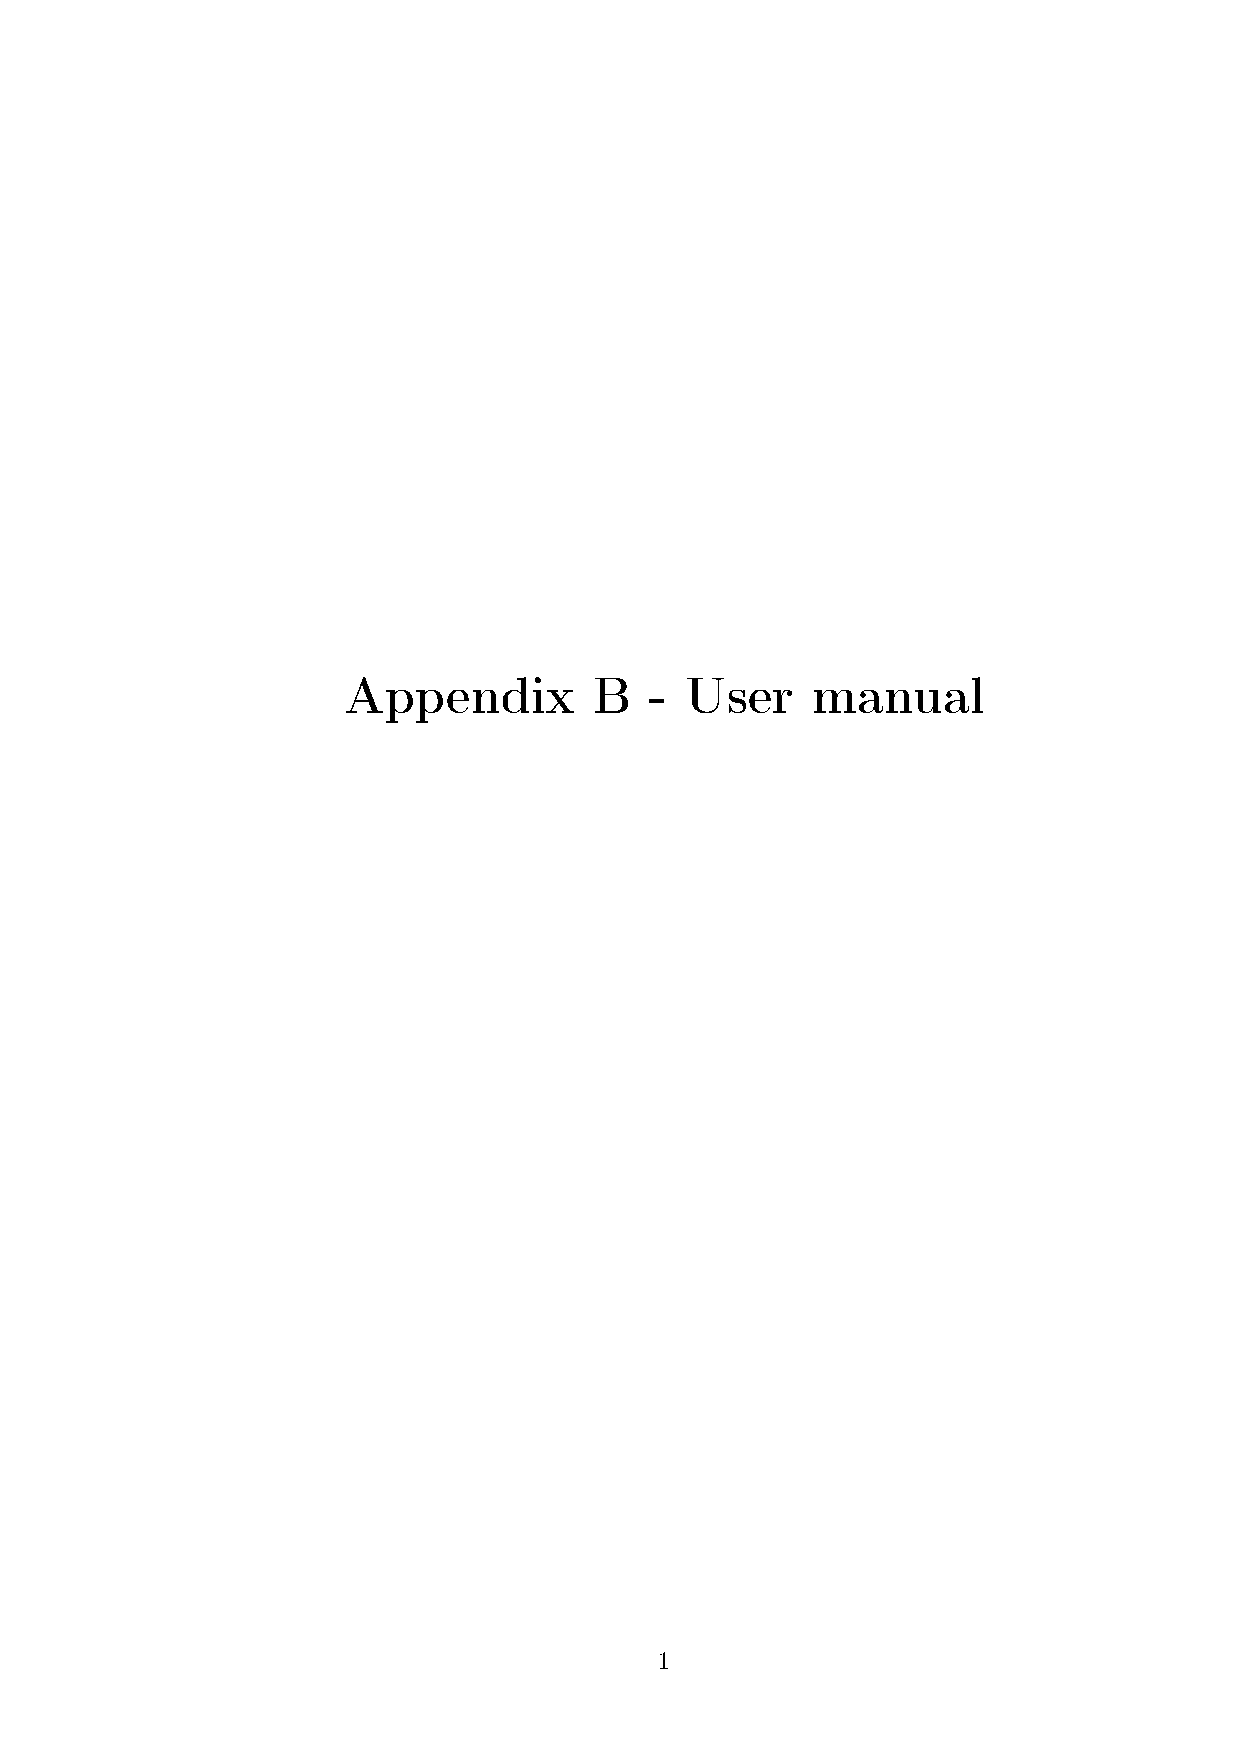
\includepdf{appendixB.pdf}




\end{document}